\chapter{Architecture design}

\section{Architecture overview}

The whole project is divided into two main parts. The purpose of the backend is to execute the Arduino code and simulate the change on the board's pinout. The purpose of the frontend is to reflect these changes on a user defined logical circuit, while offering the user control over the simulation. We chose to implement the backend in C++ and the frontend in C\#. Both backend and frontend are running in its own separate process.

\begin{figure}[h]
    \centering
    \vfill
    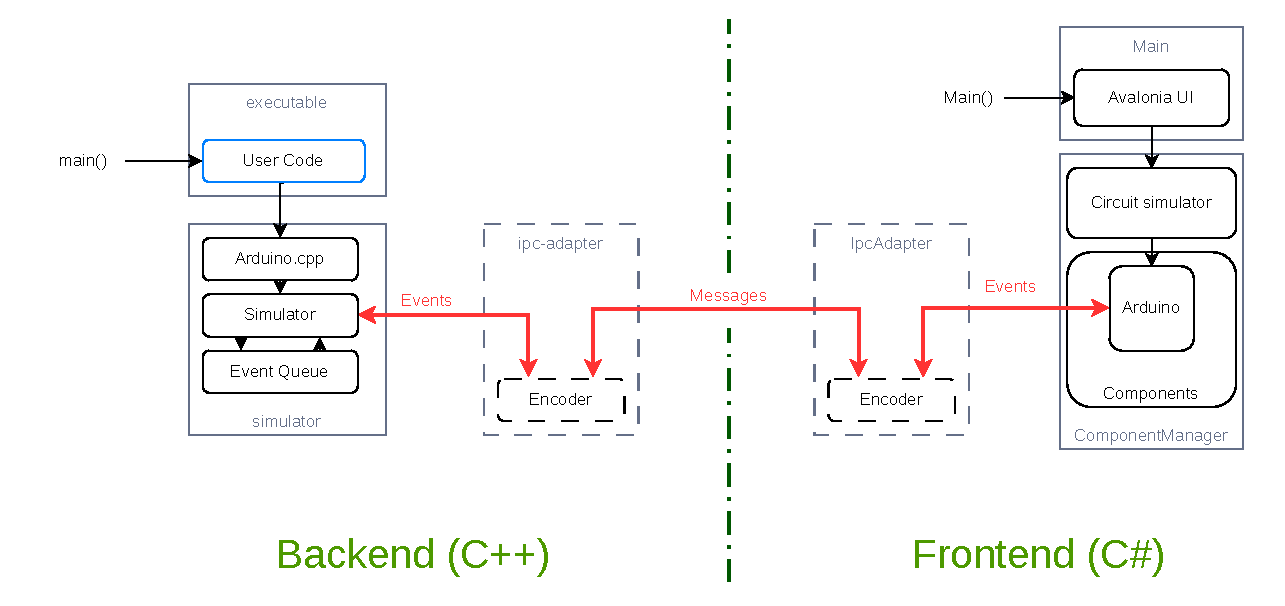
\includegraphics[width=\textwidth, keepaspectratio]{img/overall-architecture.pdf}
    \caption{Top-level architecture overview}
    \label{fig:architecture}
    \vfill
\end{figure}

The Figure \ref{fig:architecture} shows the most important systems in each process. The user coded is compiled together with the \texttt{executable} module of the backend. The declarations in the header \texttt{Arduino.h} prepended to the top of the \texttt{.ino} is implemented by a mock library \texttt{Arduino.cpp}. For each observable action an event is created and passed to the singleton \texttt{Simulator} class to compute and put into an event queue. The event is also communicated to the frontend process.

In the frontend the events are consumed by the \texttt{Arduino} component, one of several components predefined as part of the \texttt{ComponentManager} project. This project is responsible for loading user-defined components and scenes, which connect the components together in a circuit. The circuit is simulated in the same project. The user interface is implemented in the \texttt{Main} project using Avalonia UI as a framework. Interacting with the UI may invoke new events in the \texttt{Arduino} component. Those are sent back to the backend's event queue in the same manner as they were received.

The IPC Adapter is an interface implemented in each process responsible for encoding and decoding the events into a standardised format and relaying to the other process.

\section{Inter-process communication}

Implementing processes that depend on each other comes with certain challenges. Processes always run concurrently, so a variety of synchronization techniques must be applied to avoid race conditions. Before that we need to determine how will the processes exchange data. Process is a kernel level mechanism, thus approaches to handle the exchange can vary between operating systems. These mechanisms are what is called \textit{Inter-process communication}, or IPC for short.

\subsection{Considerations}
There is a technical and an engineering reason for splitting the work into more than one process.

The user must be able to have full control over the frontend user interface at all times, even while the Arduino code is being debugged. Every common debugger blocks all running threads of a process, when a breakpoint is hit. If the GUI has been part of the same process as the systems running the simulation, it would freeze and become unresponsive every time a breakpoint is hit. The only way to avoid this behavior is to separate the GUI to a different process. We want to support breakpoints in our project, as they are the most useful tool in a debugger's toolkit.

Splitting the application into multiple processes is actually a common practice among larger pieces of software. The program of each process can be written in a different programming language and thus delegated into teams with different competencies. They mark clear separation of concerns and force a solid interface design. Each process is easily swappable for another implementation with the same interface while the other processes are still running. In our case, the GUI process could be replaced by a web client, a CLI client, or an IDE add-on.

There are more than a few ways to handle IPC on every OS. The ones that we implemented are \textit{TCP stream} and \textit{shared memory}. These are among the most common approaches available both on Windows and Linux. In either case, we must clearly define what the shared data represent. Although shared memory has more flexibility than TCP, we stuck to sending discrete text or binary messages of predetermined format over time, to keep the implementation simpler and the two approaches interchangable.

Another question is what will we encode in our message. At first we encoded the full state of the simulated Arduino in \textit{snapshots} but due to its various shortcomings we later switched to sending discrete \textit{events}. So the simulator in the backend and its interpratation in the frontend both operate in terms of events, but TCP and shared memory modules only understand the notion of sending and receiving messages with very distinct interfaces. That's why we need to design an adapter in both processes and for both IPC methods that sets up the mechanism and encodes or decodes the passing messages into structured event data the simulation logic understands. The IPC adapter then informs the other systems in it's process any time a new event is received.

\subsection{Snapshotting}

In the early iterations, a snapshot of the Arduino state was sent over one message. That included the pinout state, pin modes, timer, etc. The state was periodically requested by the client with a \textit{Read} message without payload. On a change in the frontend, a \textit{Write} message with the state as payload would be sent to the server and the values of input pins would be overwritten atomically to the backend's internal state. 

This approach was easy to implement but flawed. The main issue was the frequency of reads. At lower frequencies, the system is prone to temporal aliasing. \xxx{Find temporal aliasing definition}. Some events, like very short impulses, can be missed completely. This is not much of an issue in purely combinational circuits. But we want our frontend to support stateful components, e.g. shift registers present on the Funshield, which are controlled by digital writes less than a microsecond a part.

Highering the frequency to such an extent is not viable. 

\subsection{Events}

Right now synchronization between processes is maintained by recording every significant event produced by either the backend or the frontend, and sending it to the other process. Each process is equipped with an event queue, that consumes the events in order of the least recent to the most recent. Consuming an event means invoking the appropriate function based on the type of the event with arguments stored in the event's signature. 

The Arduino object in the frontend has no logic on its own, so the only consumed events are those produced by the backend. For that reason a simple queue is sufficient, and no further synchronization is necessary. In the backend however, both simulator's and frontend's events are consumed. Sending an event to the frontend and receiving direct consequeunces of the event back can involve a significant time overhead. In the meantime the simulator produces more events that are consumed almost instantaneously. We need to ensure that the events are consumed in a valid order. We also need a robust queue implementation that isn't prone to race conditions.

An event is labeled with two timestamps. Timestamps don't have to be based on a real clock, the only requirement is that it is a non-decreasing sequence of numbers. The first timestamp sent is the simulation time, the time as perceived by the Arduino being simulated. That is time given by a clock that is started right before the \texttt{setup()} is invoked. It can be manipulated by the user by pausing or slowing down. This is to aid the user while analyzing the logs of the simulator.

The other timestamp included is \textit{Local virtual time} (LVT)\footnotemark. Each process holds its own integer value of LVT. This number is increased with newly produced events and events received from the other process. When a decision has to be made on which event to consume next (like in the case of the backend's queue), the event with lower LVT is chosen. The relation $LVT_{1} > LVT_{2}$ means that the event with $LVT_{1}$ happens after the event with $LVT_{2}$. In other words, event 1 is the consequence of the event 2 regardless of the real time passed between the events.

\footnotetext{The terminology and principles are inspired by the \textit{Optimistic synchronization} paradigm in distributed systems. In this paradigm, the events are consumed as fast as possible, and then rolled back once an event with a lower LVT than the ones consumed appears (so called \textit{Time Warp} mechanism). But Time Warp is not viable for simulating code of a high level language like C++ without custom memory management, and in our implementation it isn't even necessary.}

\subsection{TCP stream}

Messages can be sent and received through a stream of data on a TCP connection. TCP is commonly used to send data over a network, meaning backend and frontend processes can run on different machines. But listening to a connection on the same machine on the same port works just as well. TCP messages are guaranteed to arrive in the same order as they were sent.

The backend implements the TCP server, while the frontend implements the client. The implementations and design considerations behind these are very different based on the language they were written. But in both cases TCP handlers need to run on their own threads, due to how heavyweight they are. There is a buffer to which read bytes are stored from an OS network stream. These are passed as a chunk to a higher level message handler that splits the chunk into individual messages according to predetermined delimeter character. When a message needs to be sent from another thread, it is passed to the message handler where it is posted to the end of a queue and is scheduled to be processed by the OS.

There is a minor limitation of IPC over TCP that makes the debugging experience of the user's code uncomfortable. As we established, hitting a breakpoint will block all running threads of the process, including the thread with the TCP handler. When stepping through the lines of the code where events are produced, the TCP thread has to schedule posting of the message with the event, and it takes time for it to be eventually sent. In many cases the TCP thread won't be fast enough to send the message in the time the main thread progresses to the next line where a breakpoint will be hit again. As a result, consequences of the event won't be reflected in the frontend process until another one or more lines have been stepped through. This is the main reason we decided to also implement IPC with memory mapping, even though TCP is fully functional.

\subsection{Shared memory}

Memory mapping is the functionality of an operating system to relate a region of main memory 1:1 to a region in the address space of a process. This is an important idea in establishing a virtual memory of a process, but OS objects can be mapped as well. It could be either a \textit{memory-mapped file}, contents of a disk file moved to the RAM. Or it could be a special OS object called \textit{shared memory}, living in the kernel heap, specifically designed for IPC. In both cases, multiple processes can map the same memory region to their own address space. Thus they have access to the same data.

The terminology and API differ significantly between Linux and Windows, but with the use of the right libraries, the differences can be abstracted away and used as a single concept. So from now on we refer to the idea of mapping the same memory region to multiple address spaces as \textit{shared memory}.

This tool is very powerful, we can address the shared data by pointers as we would with any other data of the process. There is also no need for system calls once the the memory has been mapped. No special instructions need to be used for reading or writing and all changes are immediately visible on all of the processes that map the same region. As long as we do the writes in the simulating thread, we avoid the problem with delayed observations during debugging we encountered with TCP.

In the shared memory region, we establish a data structure that stores messages in a sequential order. We opted for a circular buffer to fully utilize the limited space of the region. There are actually two non-overlapping buffers in the same region together with a few bytes of metadata about their current state. A process consumes messages from one buffer while producing new messages to another. This is to avoid numerous race conditions that would occur while writing and reading from the same buffer while keep the synchronization mechanism lock-free.

As for the metadata, for each buffer a position after the last consumed and produced message is stored. It is important to never store references as pointers in the shared memory itself. The memory region will be most likely mapped to different addresses in each process. Because of that the \textit{producer offset} and \textit{consumer offset} are regular integers denoting the distance from the first adress of the buffer in bytes. When the offsets are equal, it means the buffer is empty. We don't care about concurrent updates of these offsets, one process changes only one of the offsets for the duration of the simulation.

\section{Backend}

\begin{figure}[h]
    \centering
    \vfill
    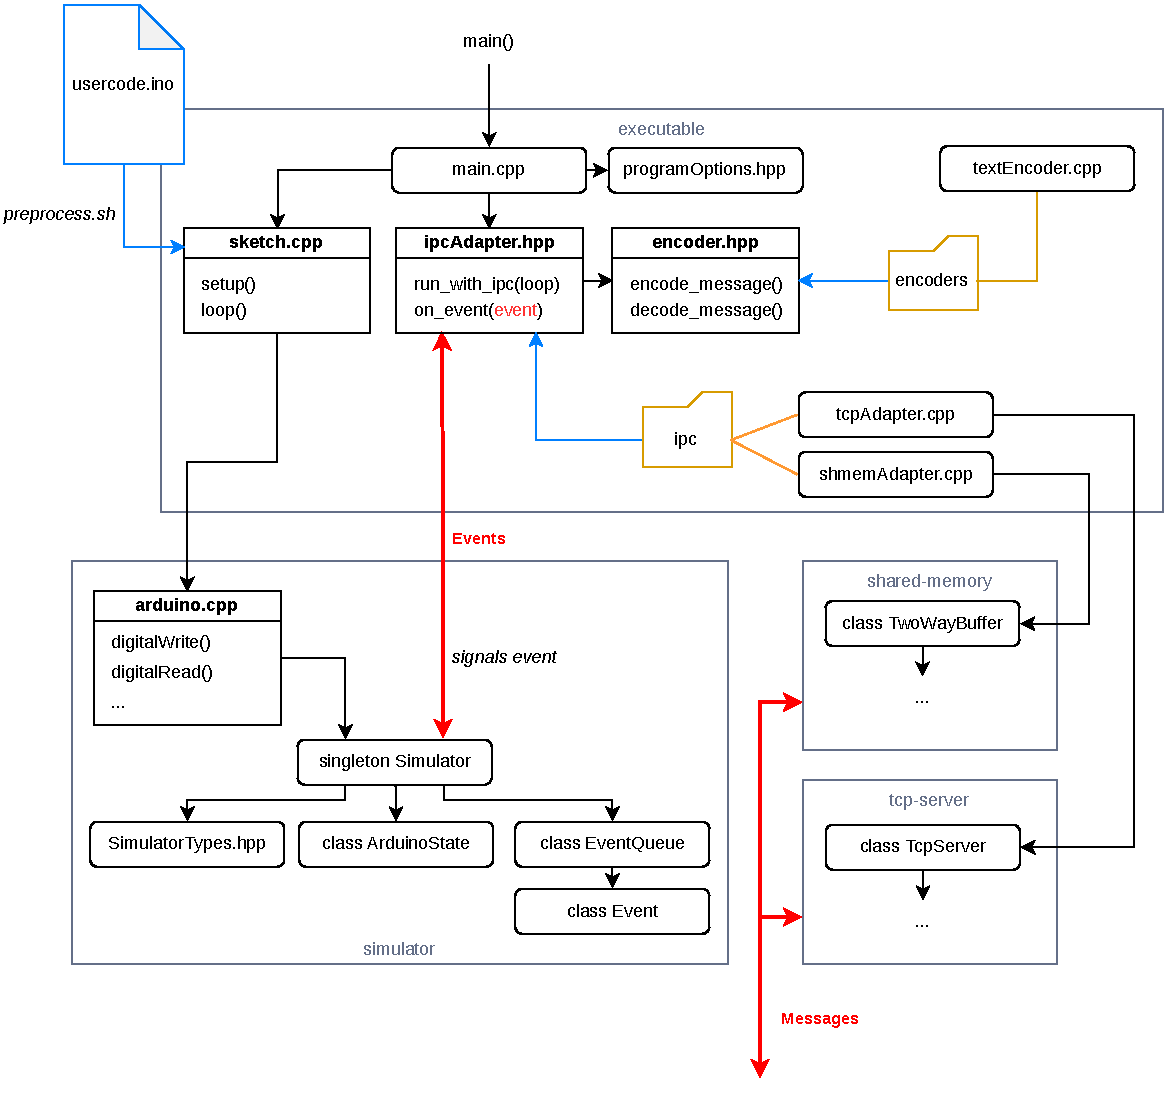
\includegraphics[width=\textwidth, keepaspectratio]{img/backend-architecture.pdf}
    \caption{Backend architecture}
    \label{fig:backend}
    \vfill
\end{figure}

The language choice for backend was obvious, the \texttt{.ino} file is a syntactically valid C++ code. We include the code in the project by passing it as an argument to the \texttt{preprocess.sh} script (\texttt{preprocess.bat} on Windows). Inside we use the \texttt{arduino-cli} tool with the right arguments to apply very light prerpocessing to the file, like adding function declarations to the top or including the \texttt{Arduino.h} header. Important additions are the \texttt{\#line} directives, which link to the definitions in the original \texttt{.ino} file. Thanks to these, breakpoints can be added to the \texttt{.ino} file and debugged as if the file itself was part of the project, completely with stepping through lines and inspection of variables. The file is then saved as \texttt{sketch.cpp} in the directory of the \texttt{executable} module where it is picked up by the CMake configuration and included in the \texttt{main.cpp}. The functions declared by the \texttt{Arduino.h} header file, like \texttt{digitalWrite} or \texttt{millis} are implemented in a custom mock library \texttt{Arduino.cpp} in the \texttt{simulator} module. Instead of instructing the AVR chip, as the real implementation would, the mock definitions create events and pass them to the \texttt{Simulator}. 

The \texttt{Simulator} singleton class is the beating heart of the backend. It is responsible for handling the events and the event queue, managing the Arduino state, logging changes and keeping track of time. It is initialized in \texttt{main.cpp} and used frequently throughout the \texttt{executable} and \texttt{simulator} modules. The \texttt{Simulator} holds the instance of the \texttt{ArduinoState} class, representing the digital states on its pins, current pin modes and the inner timer of the Arduino. It also holds the instance of the \texttt{EventQueue}, which stores both local and remote events waiting for evaluation. The \texttt{SimulatorTypes.hpp} is a header file with very few type defintions commonly used in the \texttt{simulator} module.



 

\section{Frontend}